\documentclass[12pt]{article}
\pagestyle{myheadings}
\renewcommand{\theequation}{\thesection.\arabic{equation}}
\renewcommand{\baselinestretch}{1.00}
\newtheorem{Definition}{Definition}
\newtheorem{Lemma}{Lemma}
\newtheorem{Theorem}{Theorem}
\newtheorem{Property}{Property}
\newcommand{\comment}[1]{}
\usepackage{graphicx}
\usepackage{wrapfig}
\usepackage{epsfig}
%\usepackage{subfigure}
\usepackage{subcaption}
\usepackage{caption}
%\usepackage{algorithm2e}
\usepackage{fullpage}
\usepackage{setspace}
\usepackage{comment}
\usepackage{amssymb}
\usepackage{amsmath}
\usepackage{hyperref}
\setlength{\topmargin}{0in}
\setlength{\oddsidemargin}{0.00in}
\setlength{\textheight}{9.3in} \setlength{\textwidth}{6.7in}
\newtheorem{theorem}{Theorem}
\newtheorem{definition}{Definition}
\newtheorem{notation}{Notation}
\usepackage{anyfontsize}
\usepackage{upgreek}
\usepackage{tocstyle}
\settocfeature{leaders}{\ \leaders\hrule\hfill}
\usepackage{amsmath}
\usepackage{multirow}
\usepackage{caption}

\begin{document}

\begin{titlepage}
    \begin{center}
        \vspace*{3cm}
        
        

        
        \vspace{0.25cm}
        {\Huge \textbf{Generative Adversarial Network }\par}
             

        
        \vspace{1.5cm}
        
                {\fontsize{18}{30}\selectfont \textbf{\textbf{Hamid Karimi}}}
 
        
        \vspace{.75 cm}
        
		\today        
       
        \vspace{4 cm}
        

        Michigan State University \\
        Department of Computer Science and Engineering\\
        428 South Shaw Lane \\
        East Lansing, MI 48824         
    \end{center}
\end{titlepage}


\newpage


\textbf{Loss function}.\\ Equations \ref{eq2} and \ref{eq3} show the loss functions of generator and discriminator, respectively.


\begin{equation}\tag{2}
L_D =  \frac{1}{M} \times \sum_{k} \bigg[ \log P(x_k) + \log \big(1- P(G({z_k}))\big)  \bigg] 
\label{eq2}
\end{equation}

\begin{equation}\tag{3}
L_G =  \frac{1}{M} \times \sum_{k}  \log P(G({z_k}))
\label{eq3} 
\end{equation}

$M$ is batch size, $1 \leqslant k \leqslant M$ is index of batch samples, $x_k$ is real input sample, $z_k$ is latent variable(s), $G(z_k)$ is the fake sample generated by generator from latent variable(s) $z_k$, and $P(X)$ returns likelihood of sample $X$ (either fake or real) belonging to real distribution. \\

\textbf{Model design}.\\
You can find network parameters and other settings in Table \ref{Table2}. I set number of hidden units GAN twice big as VAE's. This is because GAN was converging slower.\\

\textbf{Training and balance strategy}. \\ 
At each iteration, \textit{percentage} of improvement of generator and discriminator loss function are calculated. Then, if their absolute difference is less a threshold ($0,01)$, both of them are selected for update. Otherwise, the one which have got less improvement will be selected and the other one won't. Also, when it is discriminator’s turn, it is optimized $k$ times (here 5). Because discriminator is more likely to be left behind, I have given it more chance to keep up. Note that I am calculating percentage of improvement since last optimization. So, threshold $0.01$ corresponds to 1\%.  

\textbf{Remark 1}: at each iteration, discriminator network is called twice: once for real sample and once for generated (i.e., fake) sample. In the second call, \textit{reuse} option is true to tell tensorflow to use the same variables and not raise any error. 

\textbf{Remark 2}: discriminator and generator are optimized separately via passing their own variables to the optimizer. 
\\ 

\textbf{Results}. 

Figure \ref{GANBoth} shows visualizations of original distribution and generated one over different epochs. In epoch 401, they overlap each other quite well. Figure \ref{GANGen} plots evolution of generated Swiss-roll  at different epochs. As you can see, the shape is getting more similar to real Swiss-roll distribution. Figure \ref{GANLog} shows discriminator, generator and total loss of GAN vs training iteration and how they stabilize.\\

\textbf{VAE vs. GAN}\\ 
For this problem (i.e., generating Swiss-roll), VAE achieved better performance. VAE was faster and quality of its generated distributions was higher. \\

\textbf{Observations}
\begin{itemize}
\item An interesting phenomenon observed was GAN produces more samples from those areas of a distribution which enjoy more density. This agrees with findings of \cite{Goodfell}, GAN's original paper.
\item As the optimization proceeds, $P(G(z))$ becomes closer to $ \frac{1}{2}$. $G(z)$ is a fake sample generated by generator. In another words, discriminator is fooled and is left with no choice other than the pure random guess of $\frac{1}{2}$. Figure \ref{PGz} shows $P(G(z))$ vs iterations. As you can see, it is quite close to $\frac{1}{2}$. This is also in agreement with analytical proof shown in \cite{Goodfell}. 

\end{itemize}
 

%====================== GAN Setting Table =======================
\begin{table}[h]
\begin{tabular}{ |l|l|l| }
\hline
\multirow{4}{*}{Discriminator} & Layer1 & 200 units. Nonlinearity : tanh  \\
 & Layer2 & 200 units. Nonlinearity : tanh \\
 & Layer3 & 1 unit. Linear (yielding $P(x \in real|x)$ or $P(z \in real|z))$ \\
\hline
\multirow{3}{*}{Generator} &  Layer1 & 200 units. Nonlinearity : tanh \\
 & Layer2 & 200 units. Nonlinearity : tanh \\
 & Layer3 & 3 units. Linear (generating Swiss-roll fake points) \\ \hline
 
z dimension & \multicolumn{2}{ |l| }{2} \\ \hline
Batch size & \multicolumn{2}{ |l| }{100} \\ \hline
Learning rate & \multicolumn{2}{ |l| }{0.001} \\ \hline
Optimizer & \multicolumn{2}{|l|}{AdamOptimizer} \\ \hline
Number of Swiss-roll points & \multicolumn{2}{|l|}{10000} \\ \hline
Number of trained epochs & \multicolumn{2}{|l|}{1000} \\ \hline
Convergence epoch & \multicolumn{2}{|l|}{400} \\ \hline
Balance threshold & \multicolumn{2}{|l|}{0.01} \\ \hline
k & \multicolumn{2}{|l|}{5} \\ \hline
\hline
\end{tabular}
\caption{GAN network architecture and settings}
\label{Table2}
\end{table}

%=======================End GAN Setting Table ==================== 


%================= GAN both ================
\begin{figure}
\centering

\begin{subfigure}[t]{.4\textwidth}
\centering
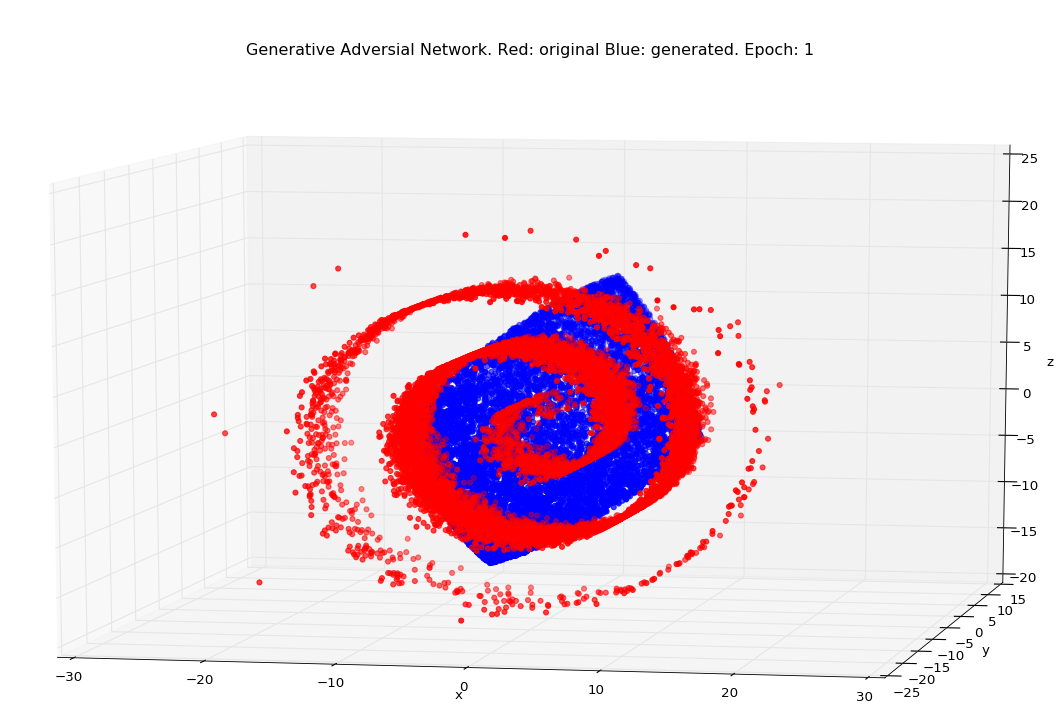
\includegraphics[width=\linewidth]{GANResults/Both1.png}
        \caption{epoch 1}
\end{subfigure}
%
\begin{subfigure}[t]{.4\textwidth}
\centering
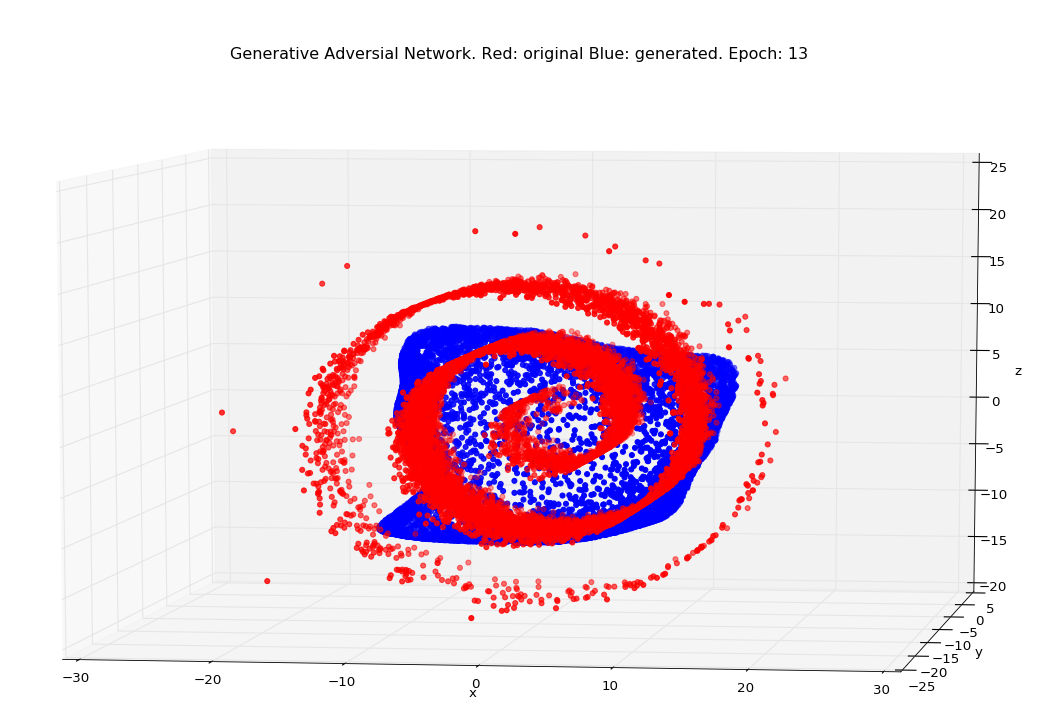
\includegraphics[width=\linewidth]{GANResults/Both13.png}
\caption{epoch 13}
\end{subfigure}
\medskip

\begin{subfigure}[t]{.4\textwidth}
\centering
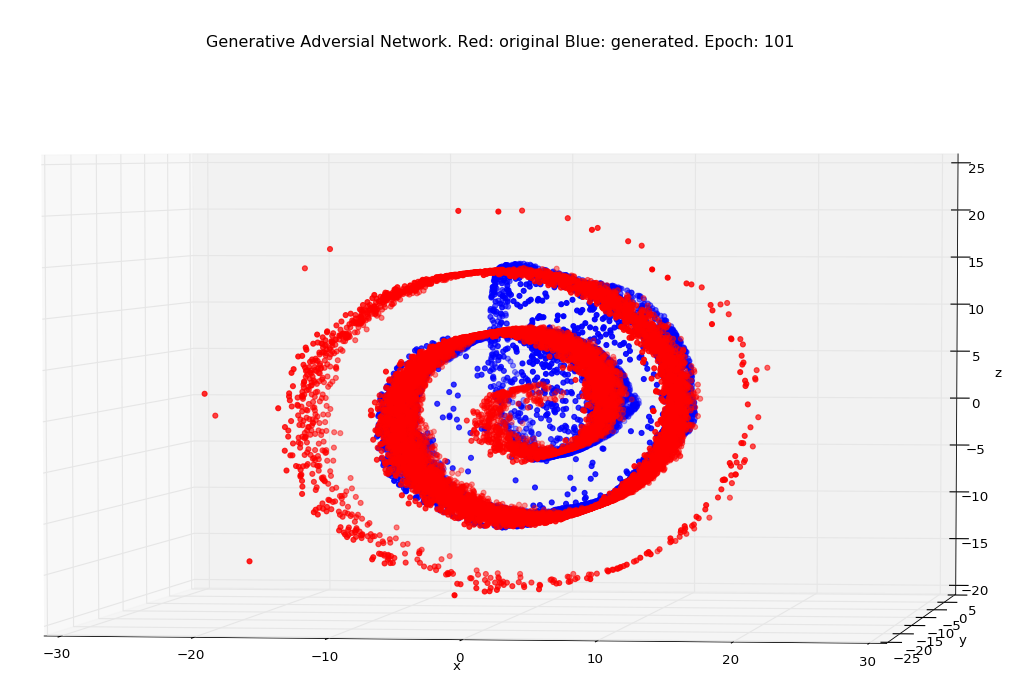
\includegraphics[width=\linewidth]{GANResults/Both101.png}
\caption{epoch 101}
\end{subfigure}
%
\begin{subfigure}[t]{.4\textwidth}
\centering
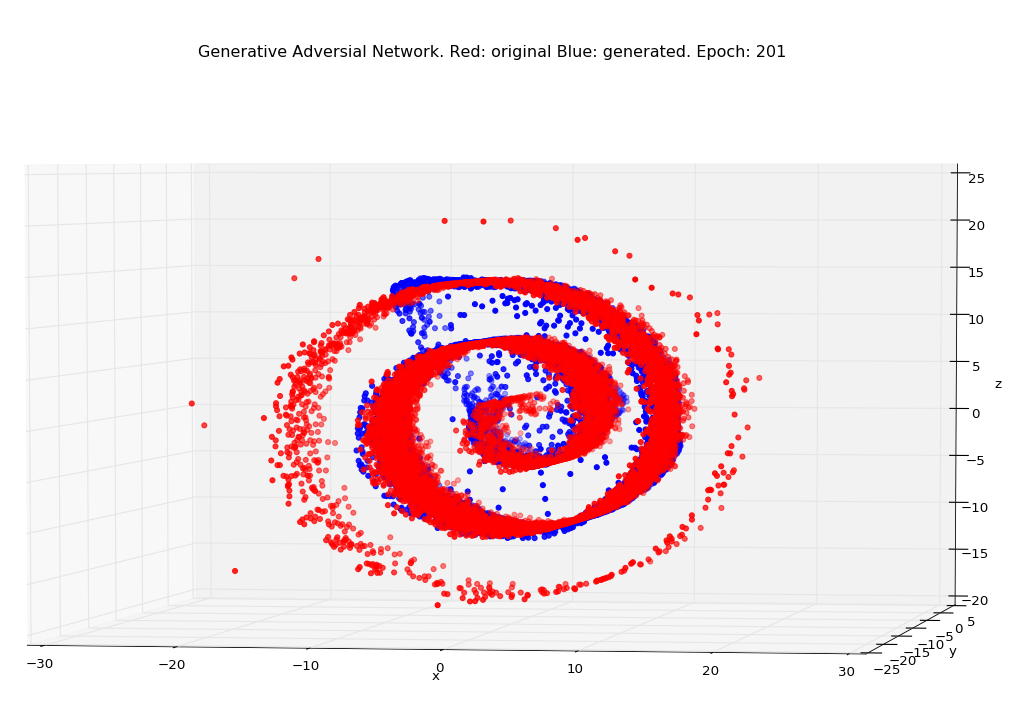
\includegraphics[width=\linewidth]{GANResults/Both201.png}
\caption{epoch 201}
\end{subfigure}
\medskip
\begin{subfigure}[t]{.4\textwidth}
\centering
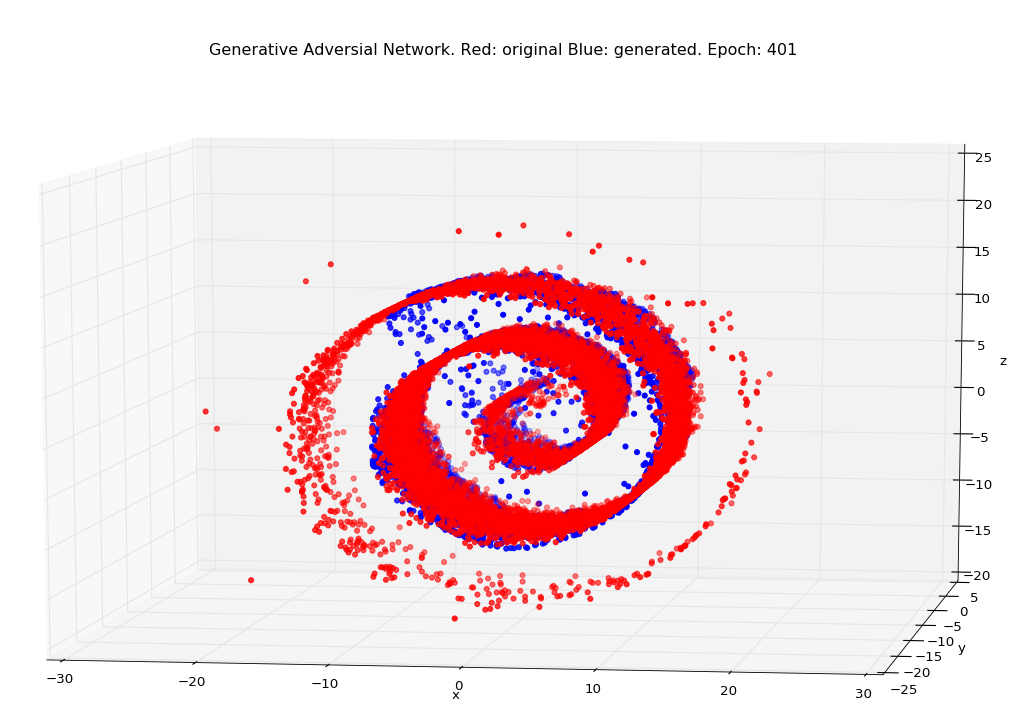
\includegraphics[width=\linewidth]{GANResults/Both401.png}
\caption{epoch 401}
\end{subfigure}%
\begin{subfigure}[t]{.4\textwidth}
\centering
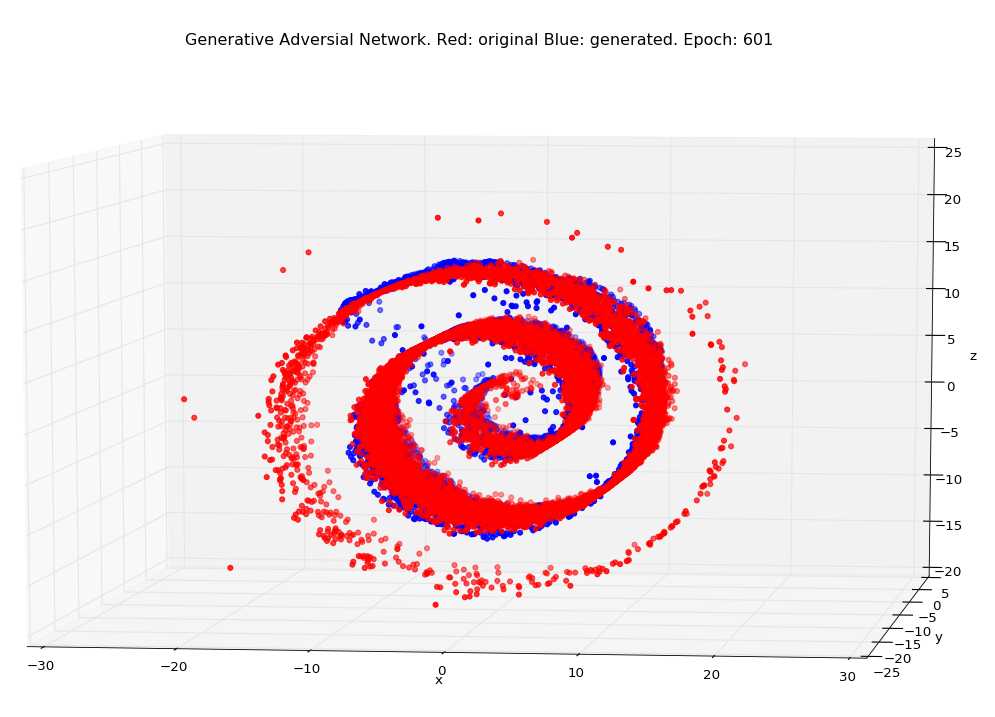
\includegraphics[width=\linewidth]{GANResults/Both601.png}
\caption{epoch 601}
\end{subfigure}

\medskip

\begin{subfigure}[t]{.4\textwidth}
\centering
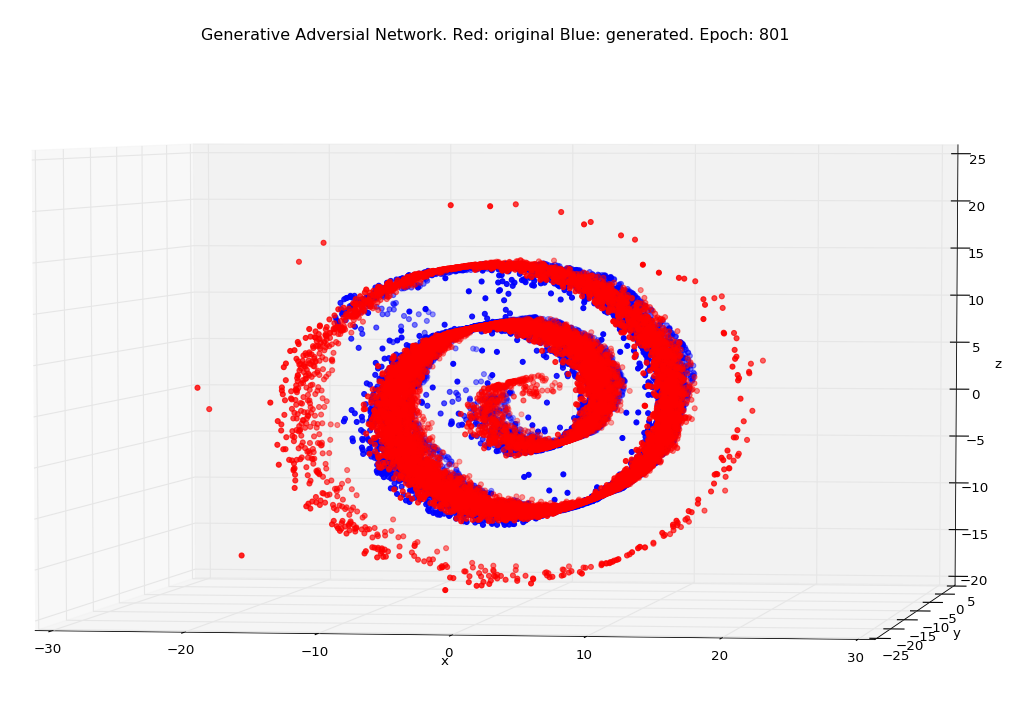
\includegraphics[width=\linewidth]{GANResults/Both801.png}
\caption{epoch 801}
\end{subfigure}%
\begin{subfigure}[t]{.4\textwidth}
\centering
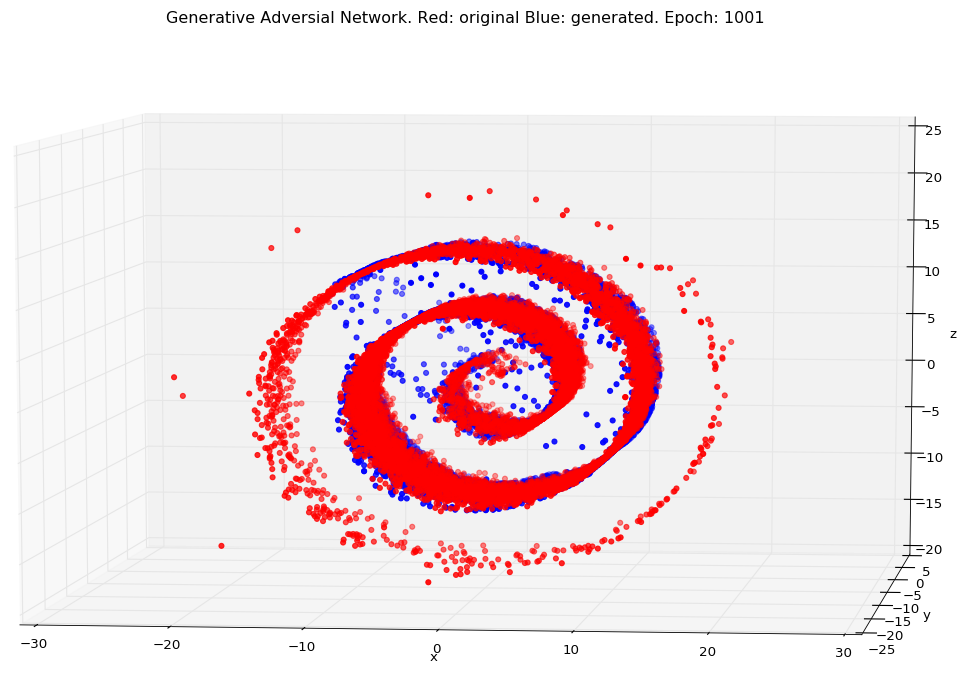
\includegraphics[width=\linewidth]{GANResults/Both1001.png}
\caption{epoch 1001}
\end{subfigure}
\caption{Generative Adversarial Network . red: original blue: generated}
\label{GANBoth}
\end{figure}
%========================= End GAN both =========================


%================= GAN both ================
\begin{figure}
\centering

\begin{subfigure}[t]{.4\textwidth}
\centering
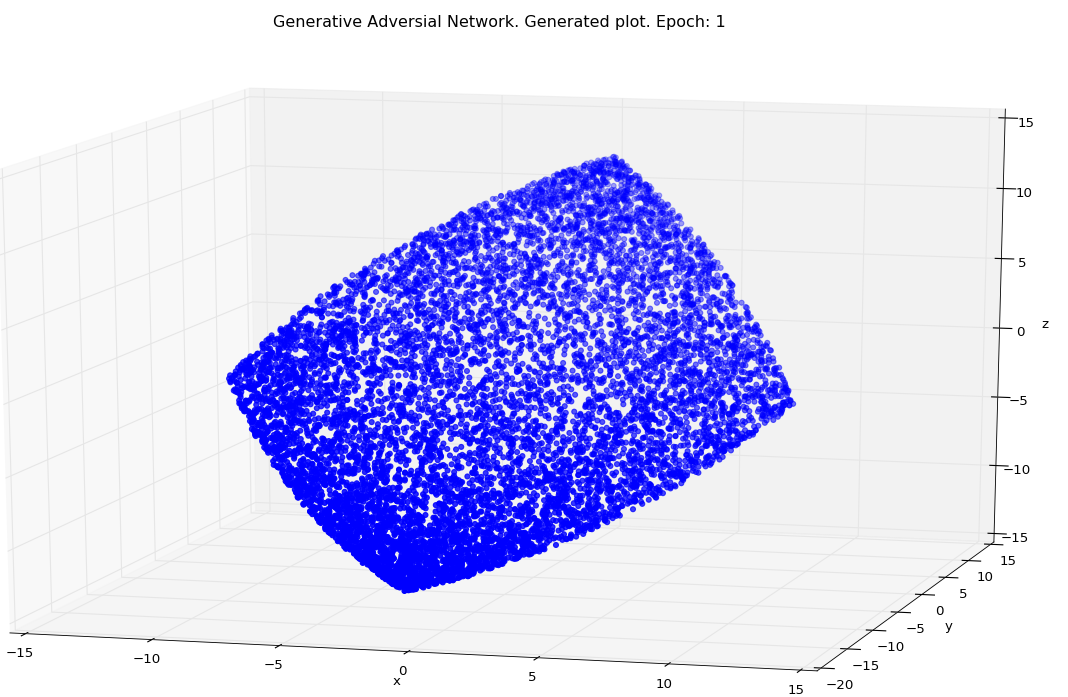
\includegraphics[width=\linewidth]{GANResults/Gen1.png}
        \caption{epoch 1}
\end{subfigure}
%
\begin{subfigure}[t]{.4\textwidth}
\centering
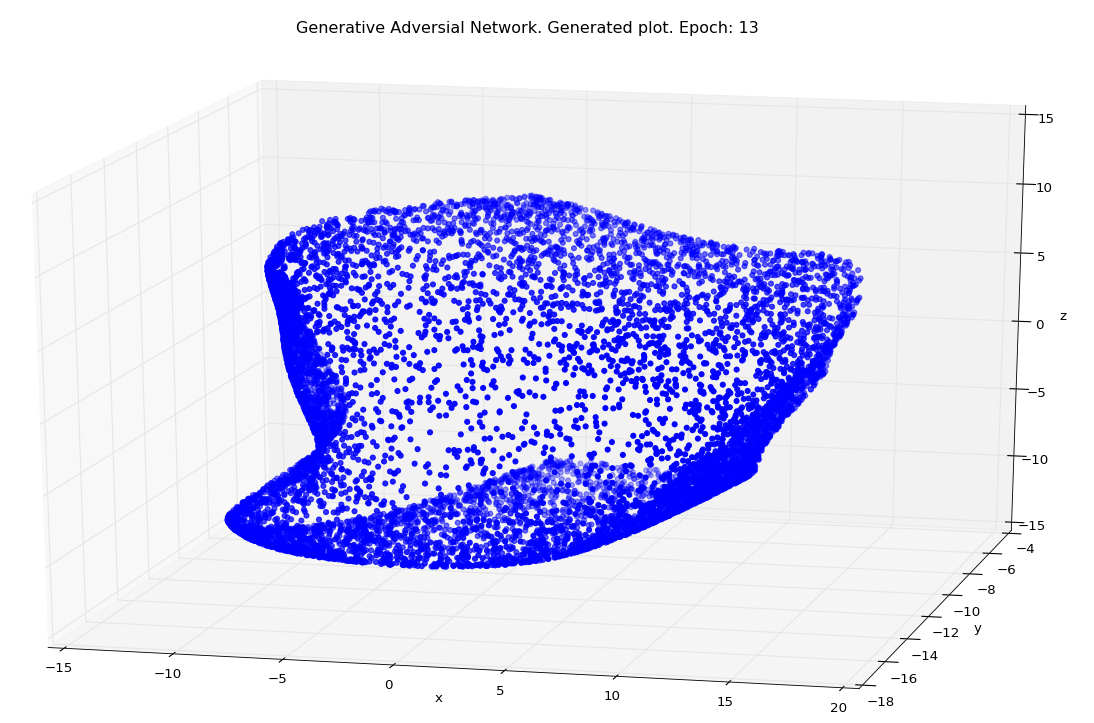
\includegraphics[width=\linewidth]{GANResults/Gen13.png}
\caption{epoch 13}
\end{subfigure}
\medskip

\begin{subfigure}[t]{.4\textwidth}
\centering
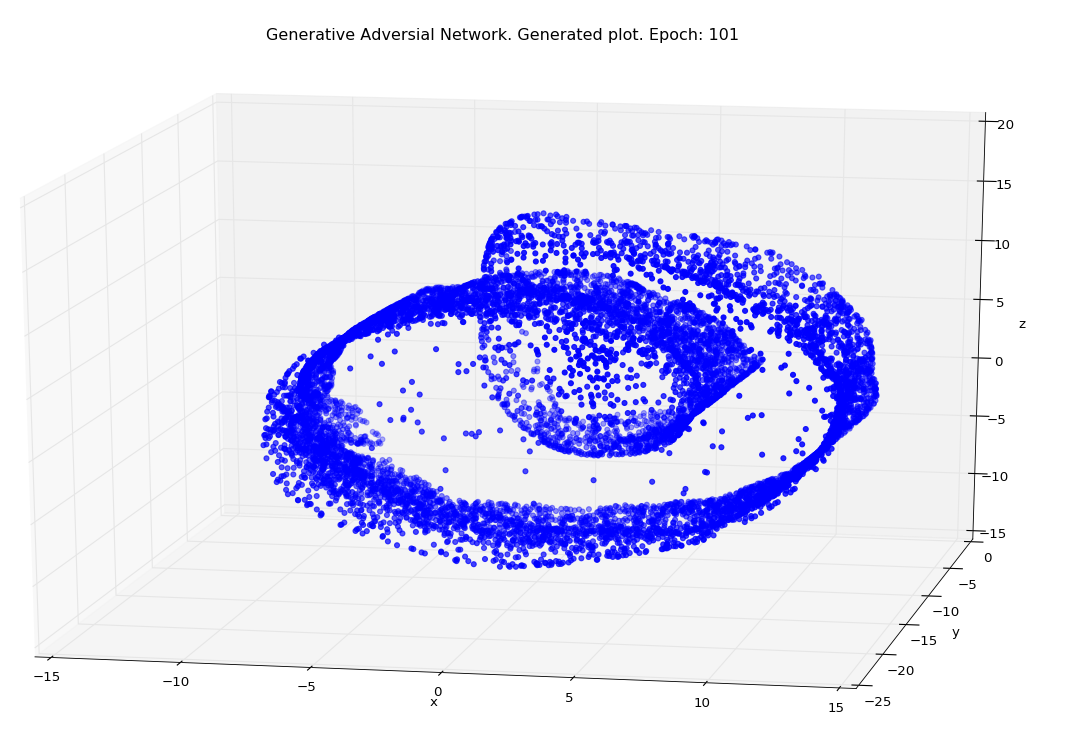
\includegraphics[width=\linewidth]{GANResults/Gen101.png}
\caption{epoch 101}
\end{subfigure}
%
\begin{subfigure}[t]{.4\textwidth}
\centering
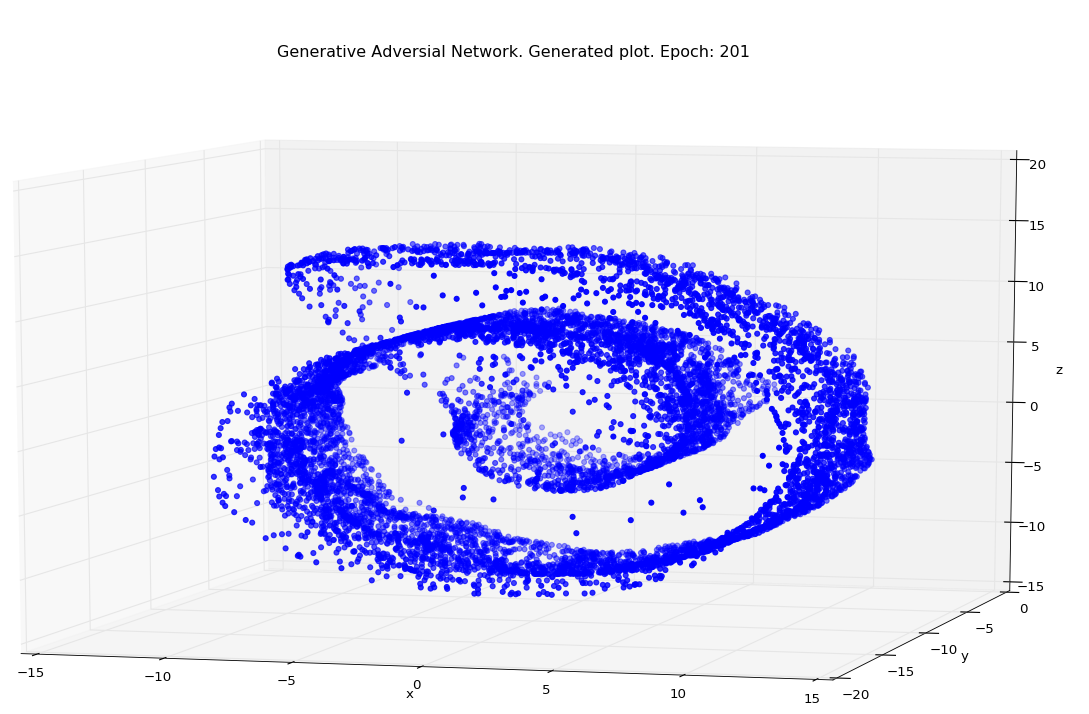
\includegraphics[width=\linewidth]{GANResults/Gen201.png}
\caption{epoch 201}
\end{subfigure}
\medskip
\begin{subfigure}[t]{.4\textwidth}
\centering
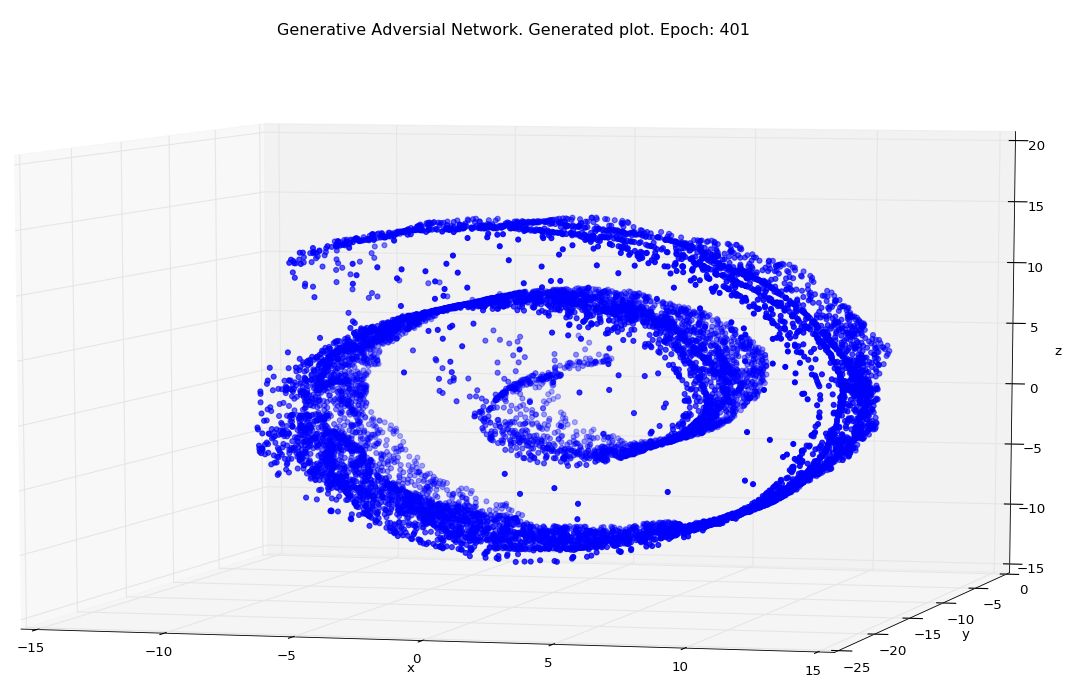
\includegraphics[width=\linewidth]{GANResults/Gen401.png}
\caption{epoch 401}
\end{subfigure}%
\begin{subfigure}[t]{.4\textwidth}
\centering
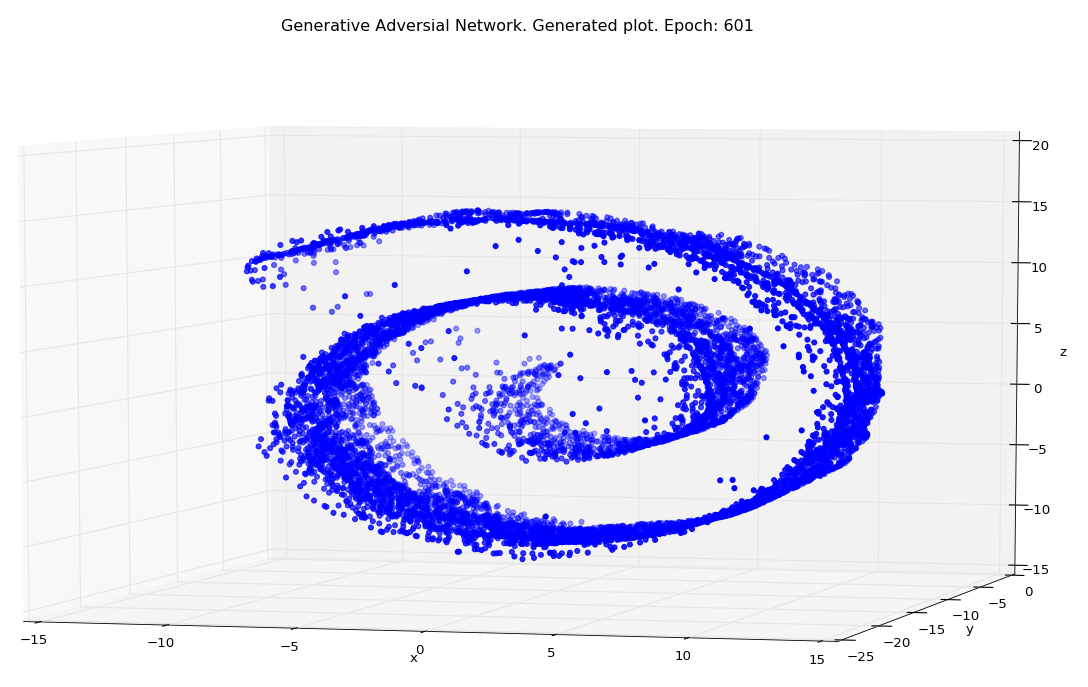
\includegraphics[width=\linewidth]{GANResults/Gen601.png}
\caption{epoch 601}
\end{subfigure}

\medskip

\begin{subfigure}[t]{.4\textwidth}
\centering
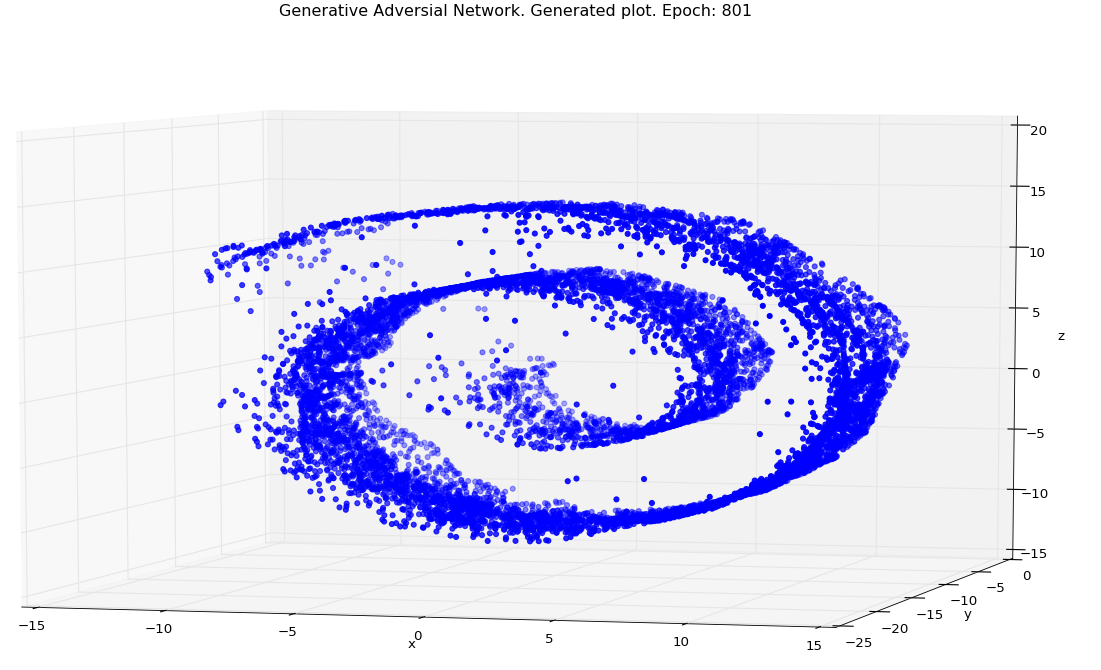
\includegraphics[width=\linewidth]{GANResults/Gen801.png}
\caption{epoch 801}
\end{subfigure}%
\begin{subfigure}[t]{.4\textwidth}
\centering
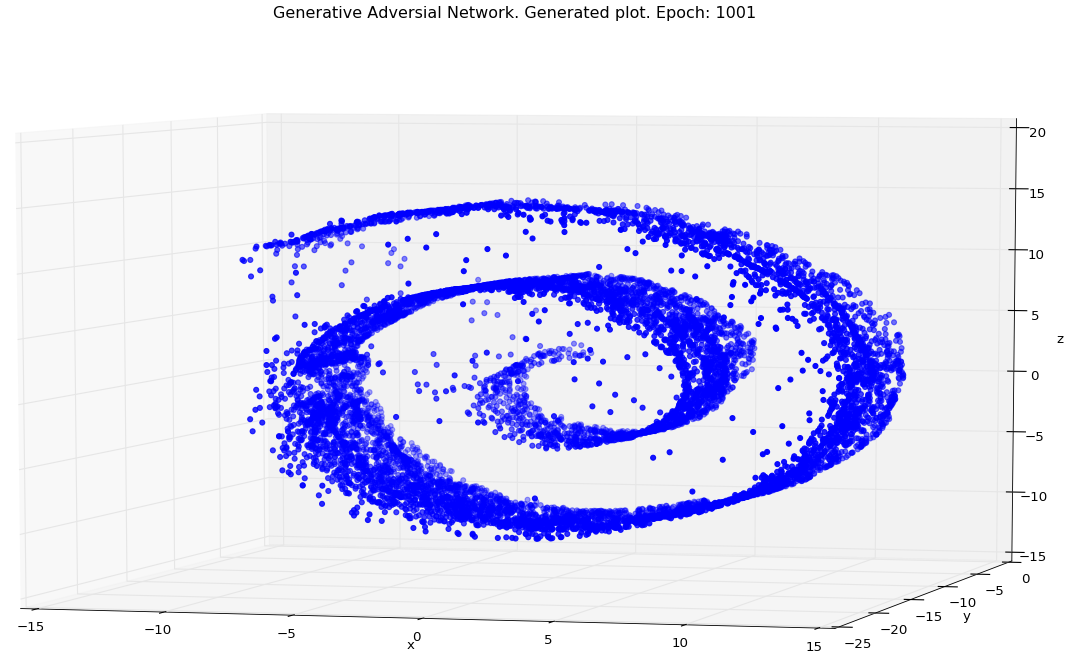
\includegraphics[width=\linewidth]{GANResults/Gen1001.png}
\caption{epoch 1001}
\end{subfigure}
\caption{Generative Adversarial Network. Generated plots }
\label{GANGen}
\end{figure}
%========================= End GAN both =========================


\begin{figure}[h]
\centering
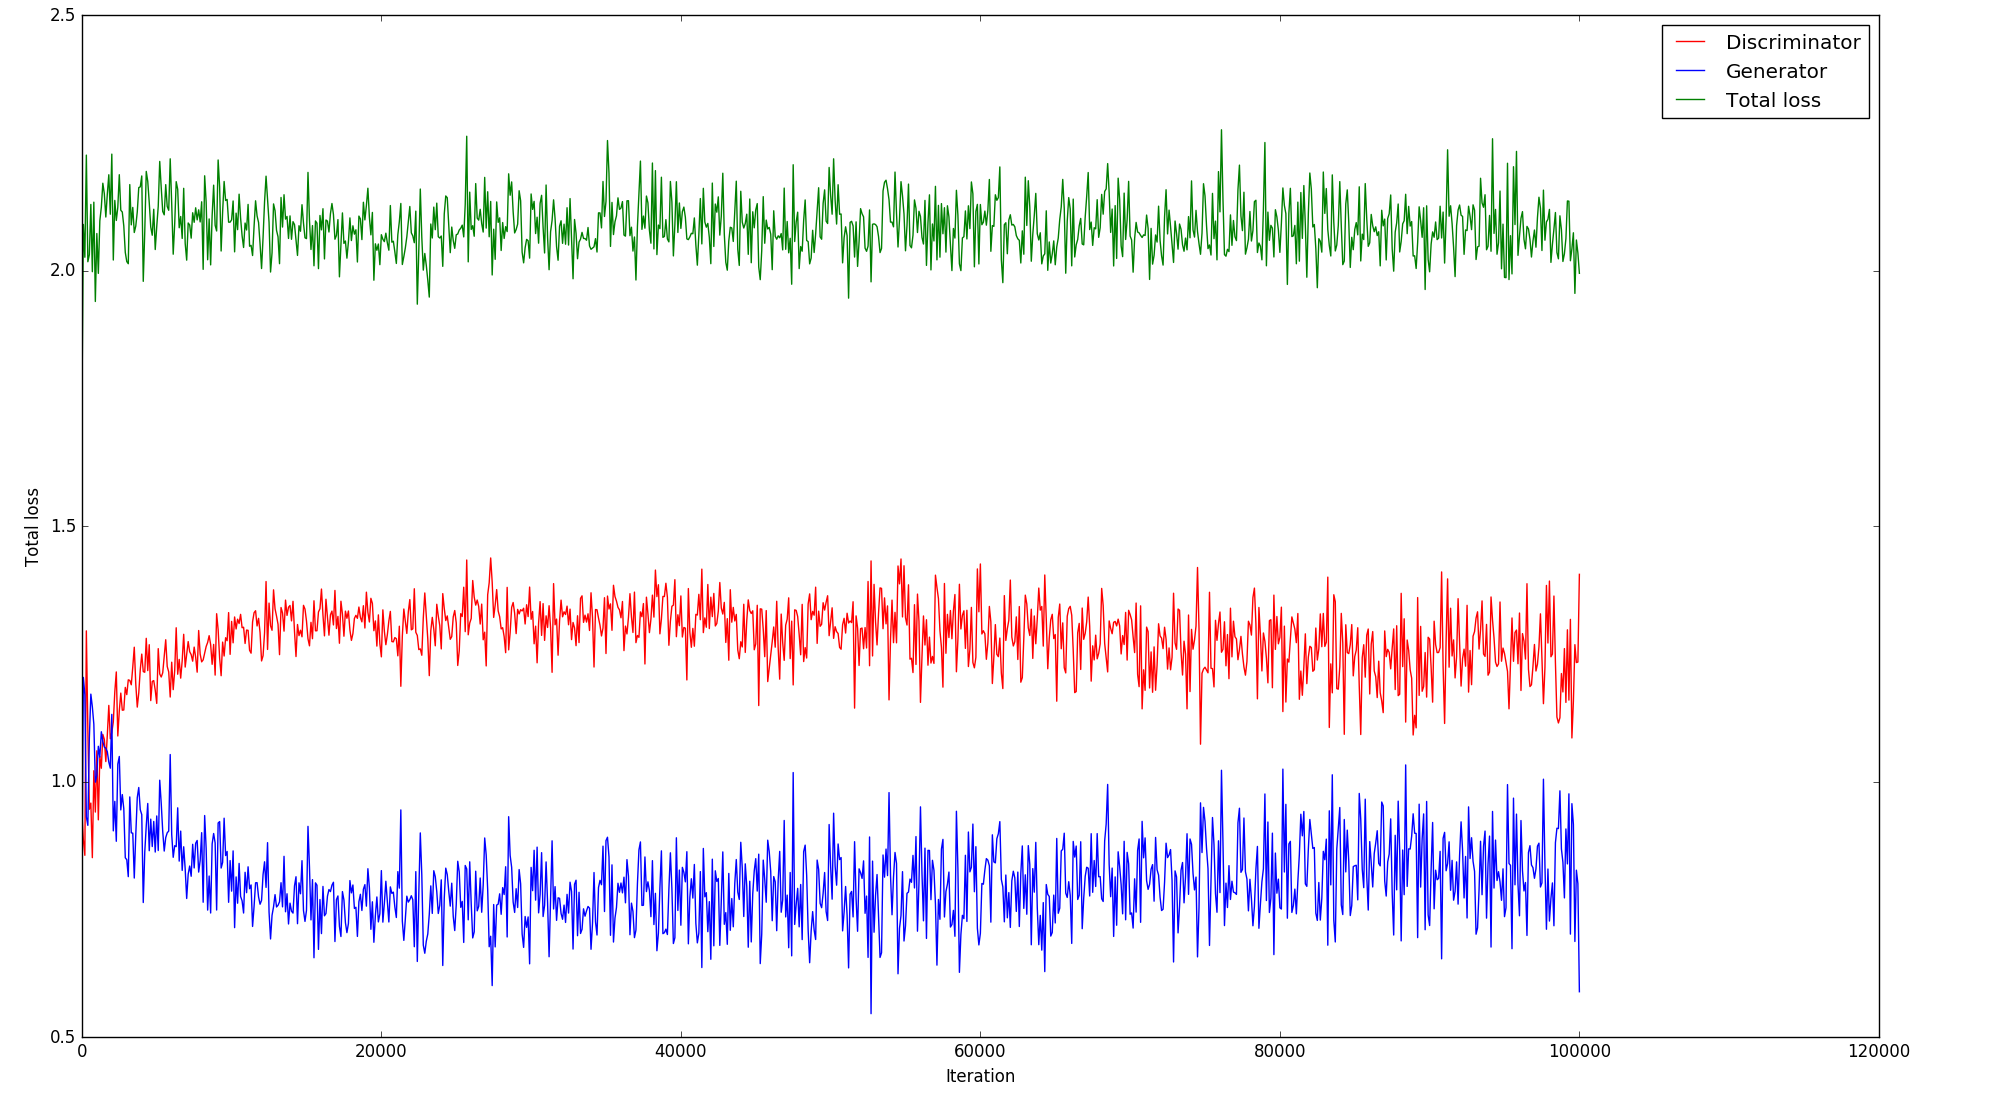
\includegraphics[scale=0.25]{GANResults/GANlog.png}
\caption{Discriminator, generator, and total loss vs. iterations }
\label{GANLog}
\end{figure}

\begin{figure}[h]
\centering
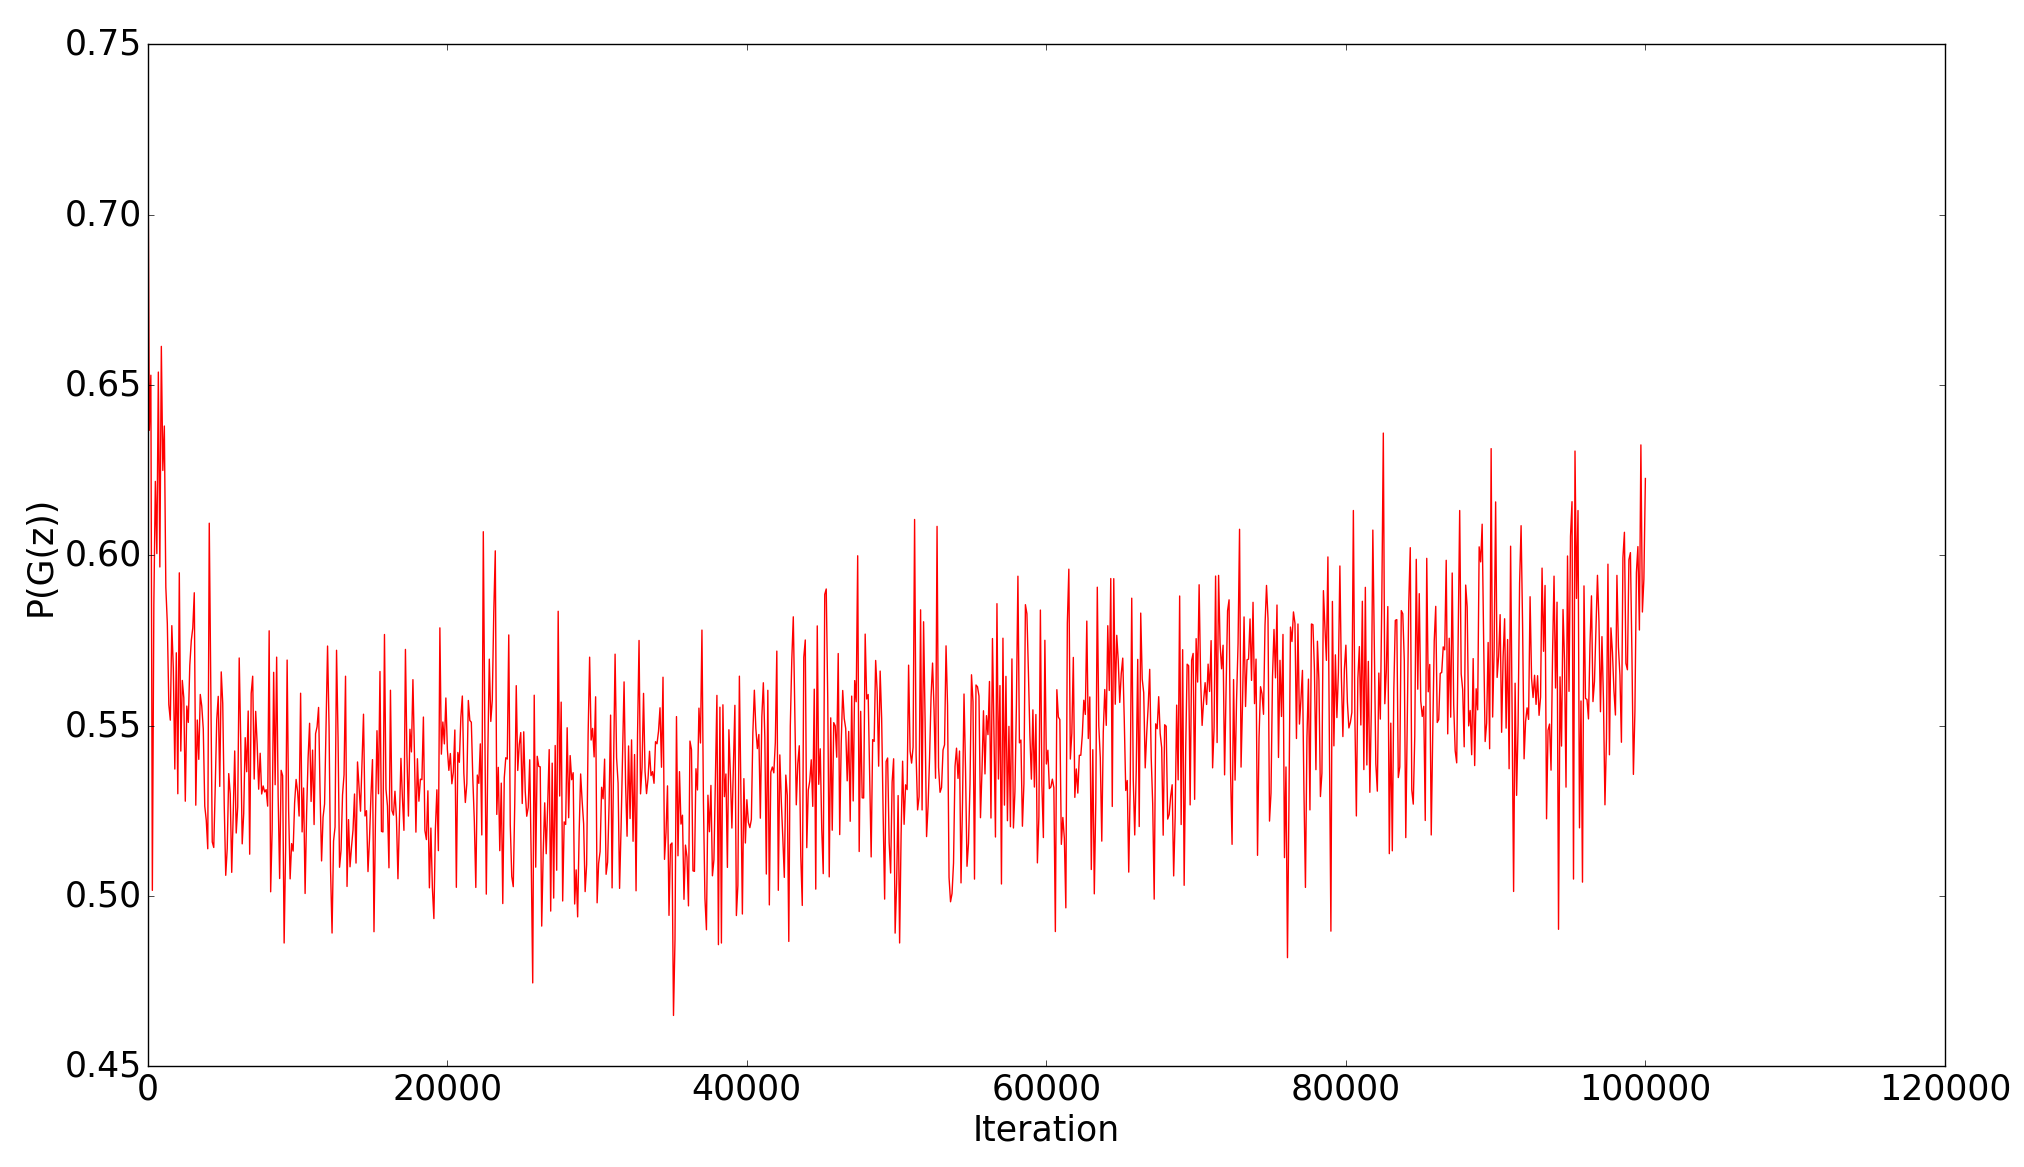
\includegraphics[scale=0.25]{GANResults/P(G(z)).png}
\caption{P(G(z)) is close to $\frac{1}{2}$ }
\label{PGz}
\end{figure}

 

\bibliographystyle{plain}
\bibliography{HW4Refs}

\end{document}


